
% Chapter 04
% !TEX encoding = UTF-8 Unicode
\chapter{Parent of Origin Effects on Gene Expression }\label{ch:poeqtl}
\section[Abstract]{Abstract}

In this chapter, I explore the impact of parental origin of genetic variation on gene expression. We perform opposite effect eQTL (oeQTL) and \emph{cis} maternal and paternal eQTL (mat-eQTL, pat-eQTL) using LCL gene expression in 306 Hutterites. We do not find any variants that have opposite effects by parental origin on gene expression with either of these two approaches. We also used a $\chi^2$ test to search for parent specific effects on reciprocal heterozygotes using parent specific gene expression and identified SNPs that have modest parent of origin eQTL effects that would need to be investigated further.

\section{Introduction}\label{ch04-introduction}
Imprinted genes have one allele silenced in a parent of origin specific manner. In humans, approximately 105 imprinted loci have been identified, many of which play important roles in development and growth\cite{Falls1999,Peters2014}. Dysregulation of imprinted genes or regions can cause diseases that show parent of origin effects, such as Prader-Willi or Angelman syndrome, among others\cite{Peters2014}. Imprinted regions have also been associated with complex traits, such as height and age of menarche \cite{Benonisdottir:2016dz,Zoledziewska:2015do}, as well as common diseases such as obesity and some cancers \cite{Peters2014}. More than 80\% of imprinted genes in humans are clustered in genomic regions that contain both maternally and paternally expressed genes, as well as genes that encode non-coding RNAs. Parent-specific expression of the genes within a cluster are maintained by complex epigenetic mechanisms at cis-acting imprinting control regions (ICRs) \cite{Kalish:2014gd}, which show parent of origin specific DNA methylation patterns and chromatin modifications.
	
Using RNA-seq and allele specific expression (ASE) we can map genes to parental haplotypes that will inform us of gene expression from parental chromosomes. With parentally mapped gene expression data, we can ask if genetic variation on the parental haplotype can influence gene expression from the same haplotype. We are not the first to look for parental genetic variation influencing gene expression: Garg et al. used gene expression in LCLs from HapMap trios to identify 30 imprinting eQTLs with parent of origin specific effects on expression including two imprinted genes\cite{Garg2012a}. However, we are the first to look for 1) parental genetic variation that can have opposite effects on gene expression, as well as 2) maternal or paternally inherited genetic variation that could affect parental gene expression on the same chromosome. 	

Here, we look for opposite parent of origin effects on total expression, as well as parent-specific expression in the Hutterites, a founder population of European descent, for which we have phased genotype data\cite{Livne2015}. We use RNA-seq from lymphoblastoid cell lines (LCLs) to map transcripts to parental haplotypes and use the parental gene expression to look for variation in \emph{cis} that would effect gene expression. Our study is underpowered to identify any opposite effect parent of origin eQTLs but we do identify a few parent of origin eQTLs where parentally inherited variation can affect parent specific gene expression from the same haplotype. 

\section{Results}\label{ch04-results}

For each of 306 individuals, the total number of transcripts at each gene was assigned as maternally inherited, paternally inherited, or unknown parent of origin. The last group included transcripts without heterozygote SNPs or SNPs without parent of origin information. Transcripts were assigned to the parentally inherited categories using SNPs in the reads and matching alleles to either the known maternally or paternally inherited alleles. All the genes analyzed had some transcripts of unknown origin (average 97.8\%, range 8.3-100\%). For each gene we assigned parental origin to an average of 1.8\% of transcripts (range: 0-34.7\%), and for each individual we assigned parental origin to an average of 1.4\% of transcripts (range: 0-1.7\%). On average, about 40 SNPs per gene were used to assign the transcripts of a gene to parent (range 1-1839 SNPs). 


\subsection{Opposite Parent of Origin eQTL (oeQTL) }\label{Opposite Parent of Origin eQTL (oeQTL)} 
Our original oeQTL identified three significant opposite effect associations but were driven by one individual's genotype. The significant associations are shown in Figures \ref{fig:oeQTL}, \ref{fig:oeQTL2}, and \ref{fig:oeQTL3}. Once we subset SNPs on having at least three individuals in at least three genotype groups, we did not find any significant results (Bonferonni corrected p-value). We were originally going to follow up significant results from this analysis with mat-eQTLs and pat-eQTLs, but proceeded with the mat-eQTL and pat-eQTL analysis anyway.


\begin{figure}[!htb]
\centering \includegraphics[width=6in]{img/ch04/fig-01-oeQTL.pdf}
\caption[Opposite Effect Association driven by one individual's genotype.]{\textbf{Opposite Effect Association driven by one individual's genotype.} Most significant opposite effect eQTL association with p-value 3.1e-09 driven by one individual with a maternal T allele and a paternal C allele.}
\label{fig:oeQTL}
\end{figure}
\clearpage

\begin{figure}[!htb]
\centering \includegraphics[width=6in]{img/ch04/fig-02-oeQTL.pdf}
\caption[Opposite Effect Association driven by one individual's genotype.]{\textbf{Opposite Effect Association driven by one individual's genotype.} Most significant opposite effect eQTL association with p-value 4.3e-09 driven by one individual with a maternal T allele and a paternal deletion.}
\label{fig:oeQTL2}
\end{figure}
\clearpage

\begin{figure}[!htb]
\centering \includegraphics[width=6in]{img/ch04/fig-03-oeQTL.pdf}
\caption[Opposite Effect Association driven by one individual's genotype.]{\textbf{Opposite Effect Association driven by one individual's genotype.} Most significant opposite effect eQTL association with p-valye 3.5e-09 driven by one individual with a maternal T allele and a paternal C allele.}
\label{fig:oeQTL3}
\end{figure}



\subsection{Single Parent eQTL (mat-eQTL, pat-eQTL)}\label{Single Parent eQTL (mat-eQTL, pat-eQTL)} 
We performed the mat-eQTL and pat-eQTL analysis, first using parent of origin normalized expression. We normalized the parental gene expression data using library sizes from the total (see Methods). However, the data was sparse and zeros drove most of the analysis. The original significant maternal and paternal associations driven by zeros in the data shown in Figures \ref{fig:mat-eQTL} and \ref{fig:pat-eQTL}. 

\begin{figure}[!htb]
\centering 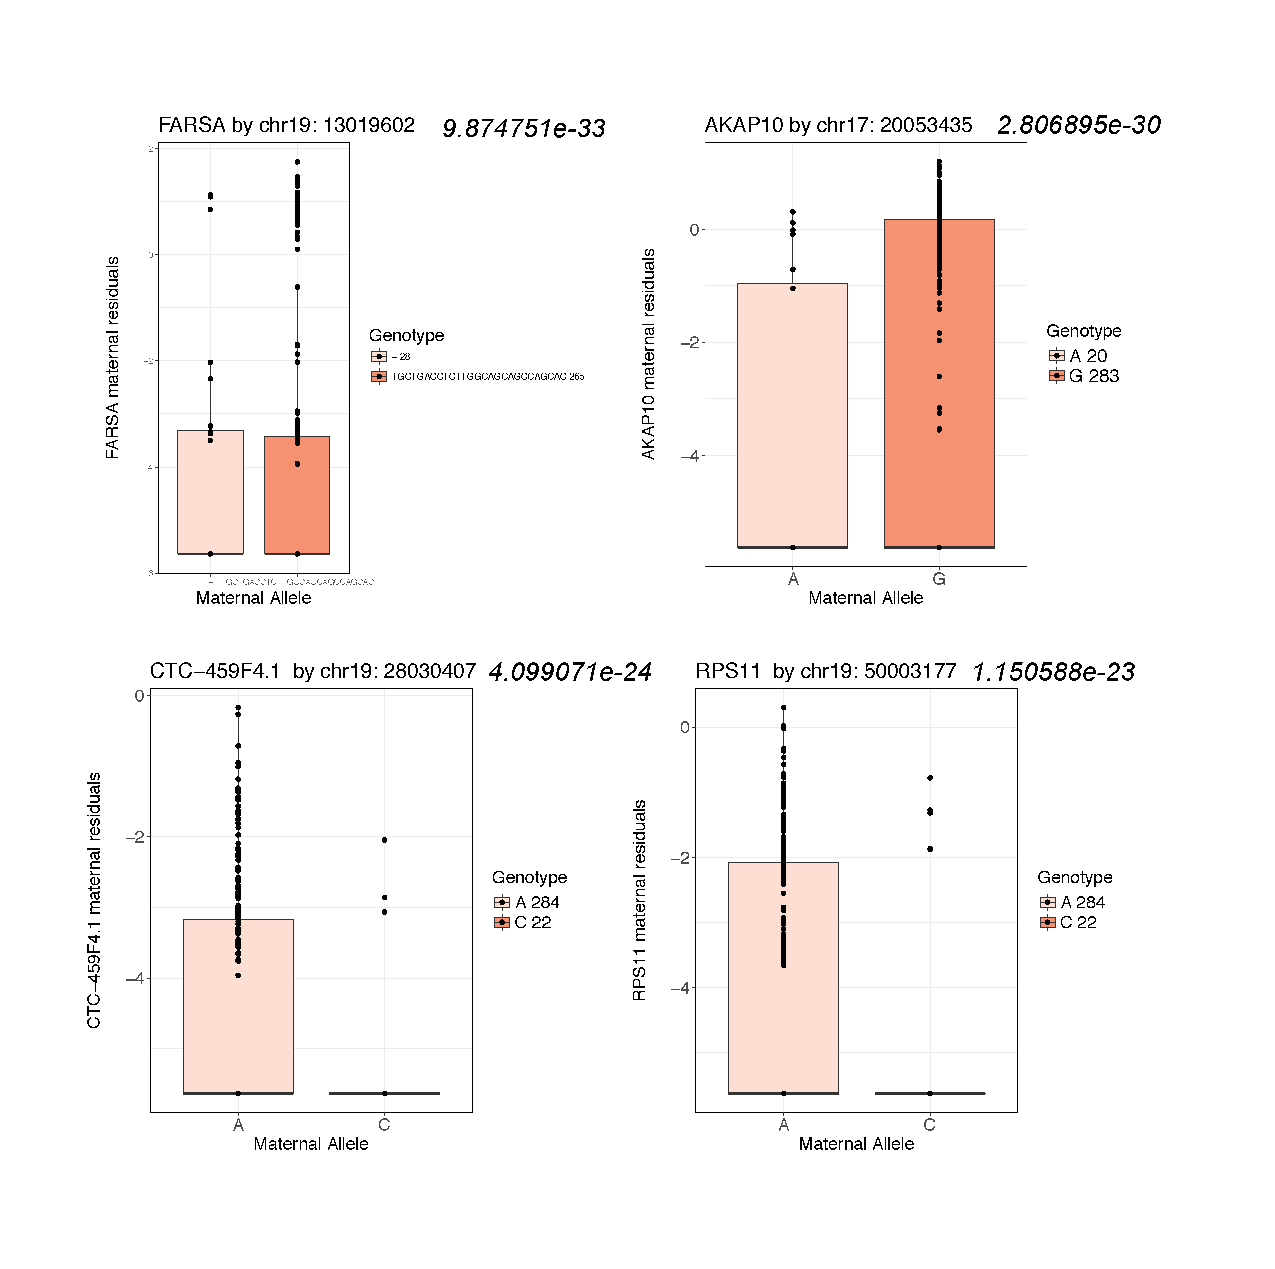
\includegraphics[width=4in]{img/ch04/fig-04-mat-eQTL.pdf}
\caption[Maternal eQTL Associations Driven by Zeros.]{\textbf{Maternal eQTL Associations Driven by Zeros.} The four most significant maternal eQTL associations. Most of the individuals have no value of expression for these genes, we see most of the genes have a median that corresponds to a value of zero after normalization. }
\label{fig:mat-eQTL}
\end{figure}

\begin{figure}[!htb]
\centering 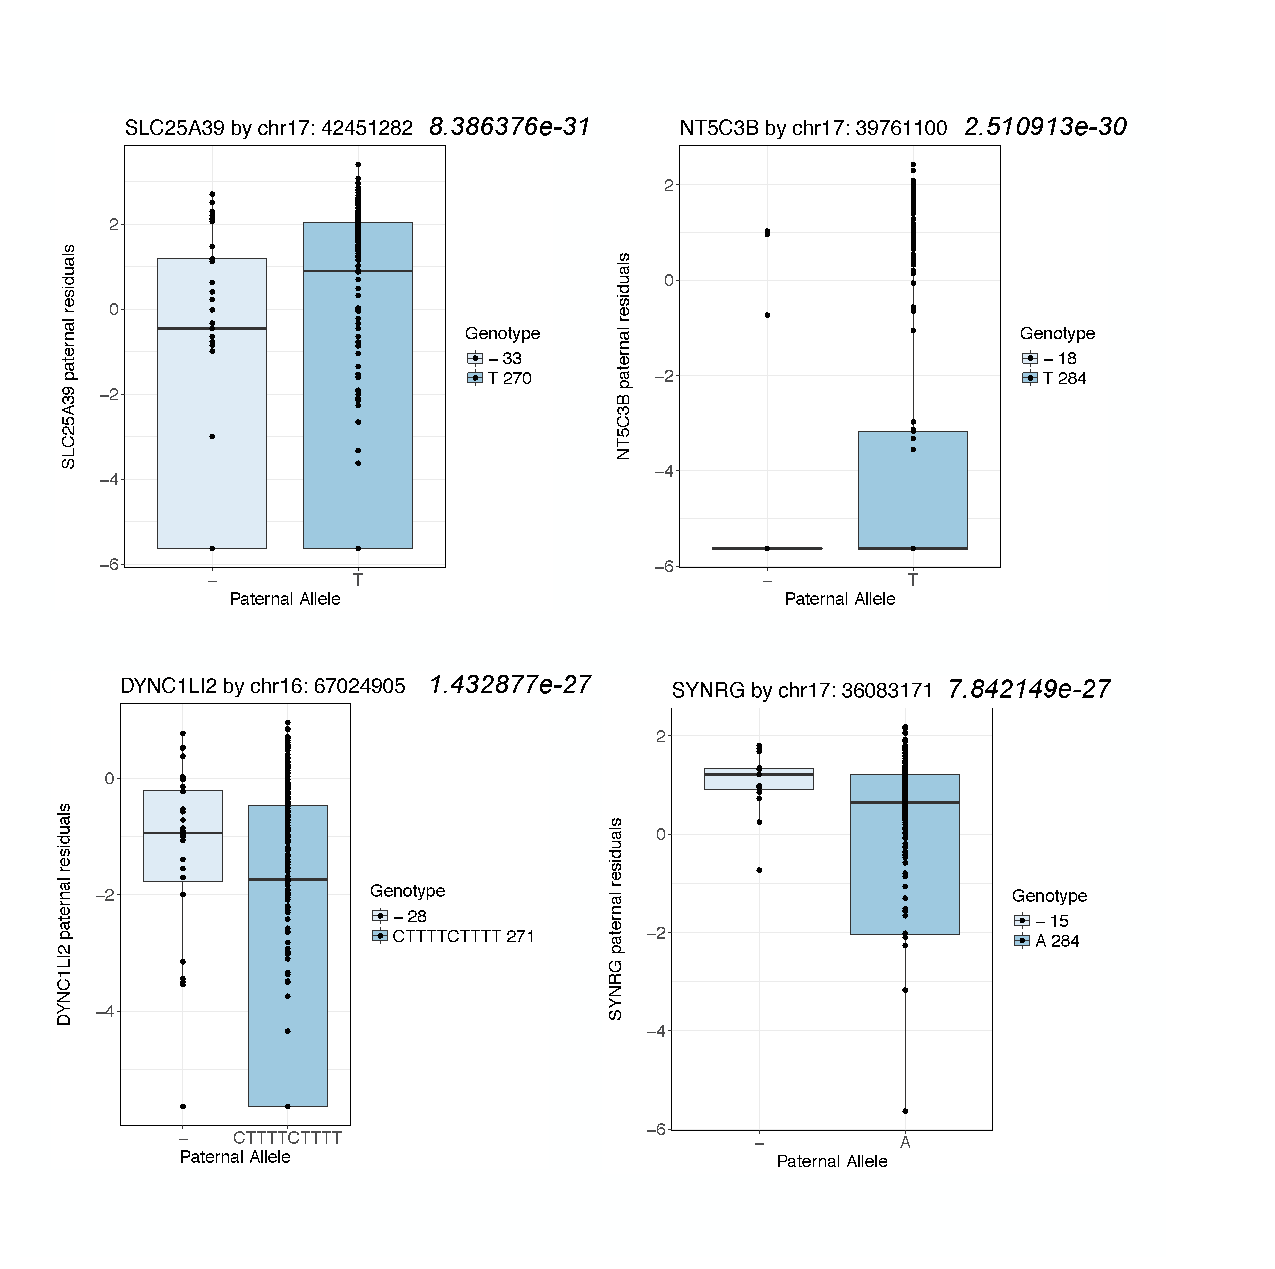
\includegraphics[width=4in]{img/ch04/fig-05-pat-eQTL.pdf}
\caption[Paternal eQTL Associations Driven by Zeros.]{\textbf{Paternal eQTL Associations Driven by Zeros.} The four most significant paternal eQTL associations. Most of the individuals have no value of expression for these genes, we see most of the genes have a median that corresponds to a value of zero after normalization. }
\label{fig:pat-eQTL}
\end{figure}


I then redid the same analysis using informative reads, removing zeros that were due to absence of heterozygous SNPs in the gene (see Methods for more detail). There were xx SNP gene pairs we could compare across both single parent eQTLs. For those significant in both, the effect sizes were all in the same direction, no SNPs had opposite effects on their corresponding parental gene expression (Figure \ref{fig:effectsizes}). The imbalance of positive and negative effect sizes in Figure \ref{fig:effectsizes} is likely due in part to the sparsity of the data, where most individuals have an expression value of zero and drive the effect size to be positive.

\begin{figure}[!htb]
\centering \includegraphics[width=5in]{img/ch04/fig-06-effectsizes.pdf}
\caption[Similar effect sizes across mat-eQTL and pat-eQTL.]{\textbf{Similar effect sizes across mat-eQTL and pat-eQTL.} }
\label{fig:effectsizes}
\end{figure}


We then compared SNP gene pairs that were significant (Bonferroni) in one parent, and not significant (p \textgreater 0.05) in the other parent (7,712 SNP gene pairs were maternally significant and not paternally significant; 10,815 paternal significant associations not maternally significant). An example in Figure . 

\subsection{Modified ASE Test}\label{Modified ASE Test} 

To detect parent of origin effects on expression another way, we did a modified ASE test (see Methods) using parental gene expression count data. Using a Bonferonni corrected p-value we identified xx significant results. The top ten significant genes with their most significant SNPs are included in Table 1. The top three genes with their most significant SNPs shown in Figure \ref{fig:top3}. Of the first four significant genes, three were imprinted genes.


\begin{figure}[!htb]
\centering 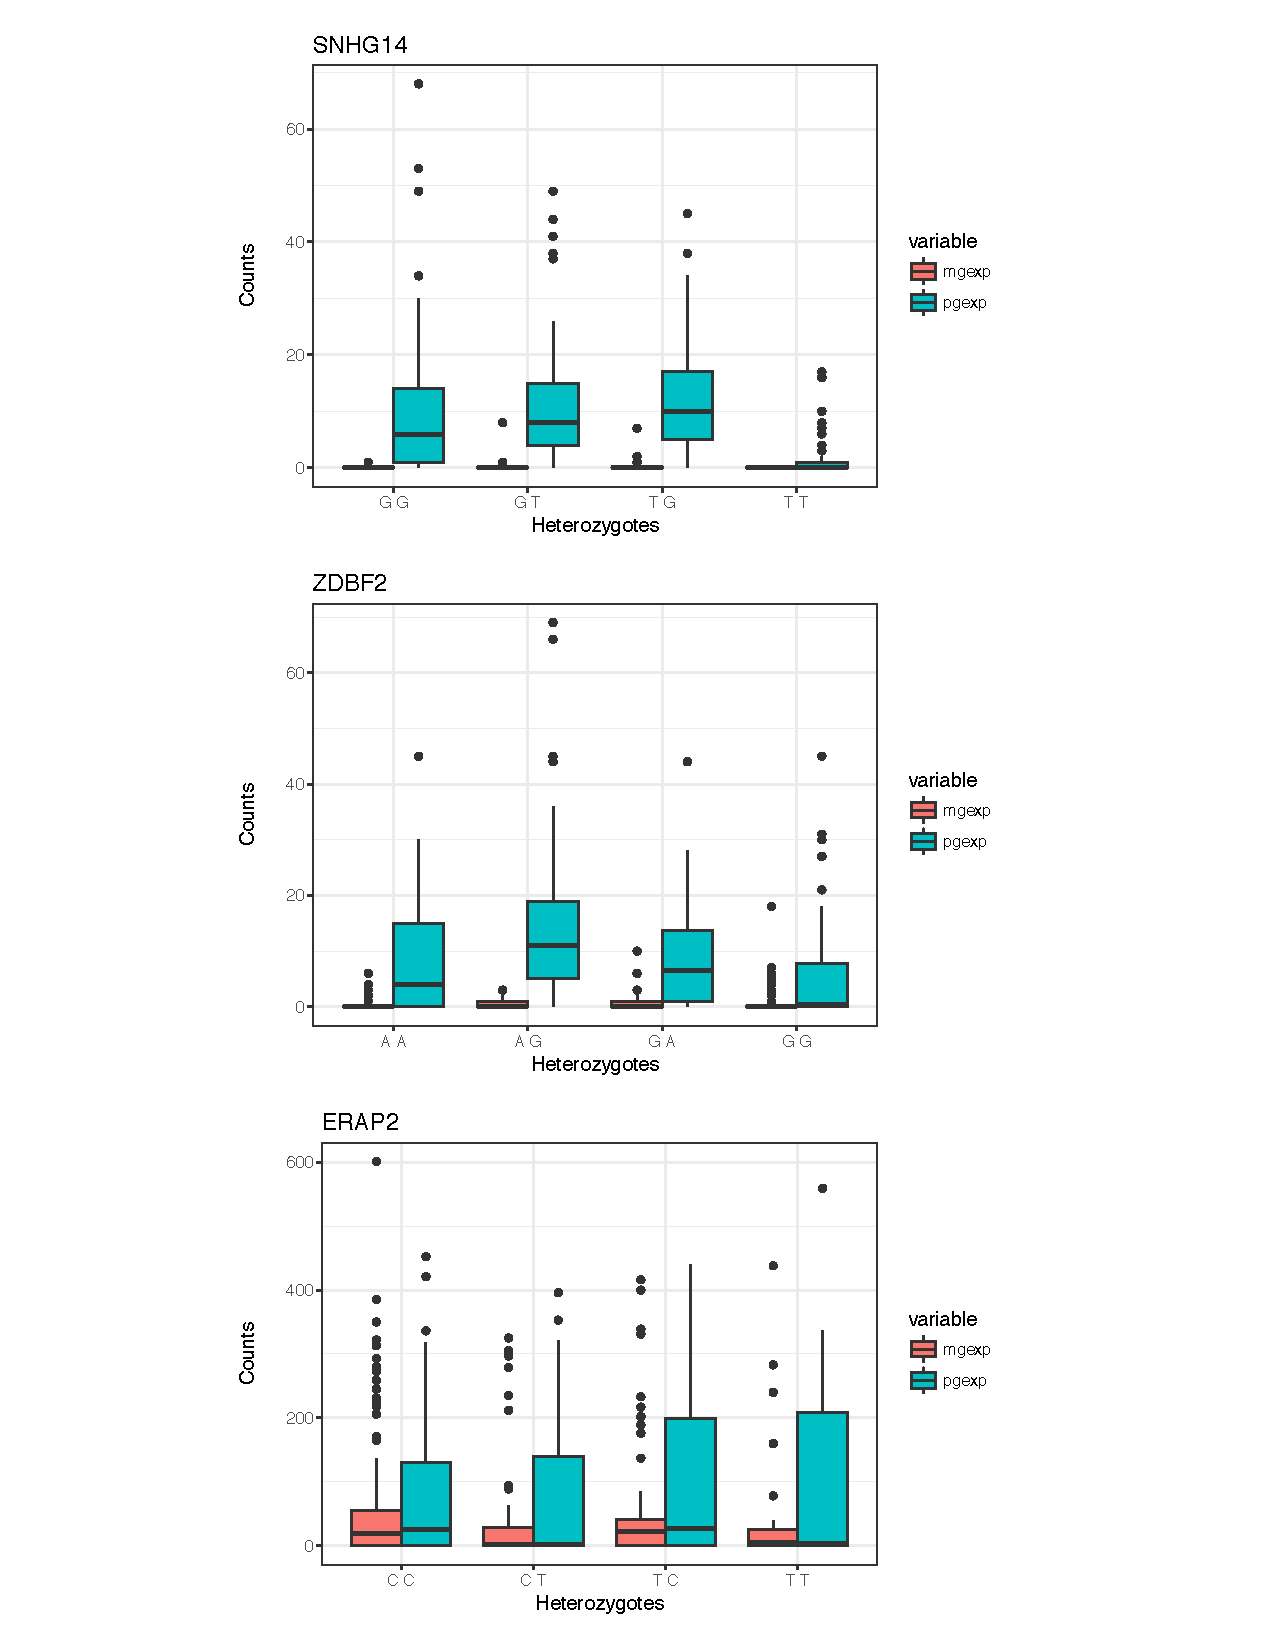
\includegraphics[width=5in]{img/ch04/fig-07-top3.pdf}
\caption[Top three significant genes from modified ASE test.]{\textbf{Top three significant genes from modified ASE test.} }
\label{fig:top3}
\end{figure}


\subsection{Modified ASE Test on Symmetrically Expressed Genes}\label{Modified ASE Test on Symmetrically Expressed Genes} 
To exclude imprinted genes in the analysis we only tested genes that did not have significant asymmetrical expression (see Methods). We identified xx significant SNPs with xx genes using Bonferonni (p-value xx). The two most significant genes with symmetric expression that are also significant in this test are plotted with their most significant SNPs in Figures \ref{fig:SEC22B} and \ref{fig:ZMAT3}.


\begin{figure}[!htb]
\centering \includegraphics[width=5in]{img/ch04/fig-09-SEC22B.pdf}
\caption[SEC22B.]{\textbf{SEC22B.} }
\label{fig:SEC22B}
\end{figure}


\begin{figure}[!htb]
\centering \includegraphics[width=5in]{img/ch04/fig-10-ZMAT3.pdf}
\caption[ZMAT3.]{\textbf{ZMAT3.} }
\label{fig:ZMAT3}
\end{figure}



\section{Discussion}\label{ch04-discussion}

Previous studies using parental alleles and gene expression have identified imprinted genes and genetic variation that affects quantitative traits\cite{Zoledziewska:2015do,Baran:2015cx,Benonisdottir:2016dz,Garg2012a}, but none to our knowledge have looked at how genetic variation can impact parent of origin expression.

Here we used parental specific gene expression in 306 Hutterite individuals to characterize genetic variation on parental expression. We first performed a parent of origin opposite effect eQTL (oeQTL) using total gene expression. We then did a maternal and paternal eQTL on maternal and paternal gene expression (mat-eQTL, pat-eQTL), respectively. We finally looked for parent of origin effects among reciprocal heterozygotes.

Our opposite effect model has been successful in identifying opposite effects of parentally inherited variants on quantitative traits in the Hutterites but we weren't able to find any with LCL gene expression. These could be due to a number of limitations of this study, including sample size and tissue studied. We also performed our \emph{cis} mat-eQTL and pat-eQTL. This test identified known significant eQTLs as they would show up in both mat-eQTL and pat-eQTL results since the effect does not depend on the parent of origin. None of the variants compared across the two showed opposite effects by parent of origin. We were not able to find any maternal or paternally only effects on gene expression without breaking down the data further.

We found that most of the negative results were driven by sparsity in the data. Zeros in gene expression could be due to two factors: 1) no heterozygous/parent of origin SNPs in the gene such that homozygous reads could not be assigned to a parent, or 2) there are heterozygous SNPs in the genes but there are no reads. We assigned genes for individuals that did not have any heterozygous SNPs as missing and kept the values for those with at least one heterozygous site in a gene. This resulted in different numbers of individuals and genes to be tested. This provided a more conservative and informative data set but we did not find any significant maternal or paternal only effects on gene expression.

Finally, we performed a modified ASE test among reciprocal heterozygotes to identify effects of parental variation on gene expression. The missing gene expression (i.e. uninformative) for some individuals, decreased the numbers of reciprocal heterozygotes we could test for each gene.

These few results could be due to many limitations of our study. Although we were able to determine the parent of origin for many transcripts in the Hutterites, we could not assign every RNA sequencing read to a parent due to lack of heterozygous sites or missing parent of origin information for alleles. A lot of genes were missing parental gene expression resulting in very sparse data. Second, we conducted these studies in LCLs, and therefore could only study parent of origin effects in LCLs and would miss any effects in other tissues or developmental time points. Additionally, our models to test for parent of origin eQTL effects are decent but could be much improved, such as to model over-dispersion in gene expression.

In summary, we did not identify any genetic variation that has opposite parental effects on parental specific or total gene expression. We did identify SNPs with parent of origin eQTLs that were not affecting imprinted genes even though our data is still a bit noisy and underpowered. More sequencing and better modeling could potentially identify more genetic variation that impacts parental gene expression.

\section{Methods}\label{ch04-methods}

\subsection{Genotypes and Sample Information}\label{Genotypes and Sample Information}
LCL RNA-seq transcripts for 306 individuals were mapped to parental haplotypes as in Chapter \ref{ch:imprinted}. We used the measures of total as well as maternal and paternal expression in this study. We used multiple approaches to characterize parent of origin effects on gene expression.
To be conservative, we used 306 Hutterite individuals for which we have parental genotypes and tested SNPs for which we have at least three individuals in at least three of four parent of origin genotype classes (such that we have at least three individuals in at least one heterozygote category and one heterozygote individual will not drive our analysis). We used QCed SNPs with MAF \textgreater 5\%.

\subsection{RNA-seq QC}\label{RNA-seq QC}
Multiple approaches required different QC method. For the total gene expression, we used normalized gene expression. First, we removed lowly expressed genes with a log count per million (cpm) greater than 1 in at least 20 individuals.The R/Bioconductor package edgeR was used to convert the RNA-seq counts to log2 TMM-normalized CPM values\cite{Robinson:2010dd,Robinson:2010cw}. Technical covariates correlated with gene expression Principal Components were regressed out (RIN, DNA concentration, RNA concentration, Flowcell/Lane). 

\subsection{Parent of Origin Expression QC}\label{Parent of Origin Expression QC}
Maternal gene expression was used as both counts and as normalized gene expression. Maternal gene expression counts were used directly from STAR gene count output\cite{Dobin:2002by} subsetted on genes included in the total gene expression analysis. 
Normalized maternal expression was calculated using similar to total gene expression using edgeR and converting RNA-seq counts to log2 TMM normalized CPM values using normalization factors (library sizes) from the total gene expression (maternal gene expression too sparse on it's own). 
Same method was used to get paternal gene expression counts and normalized paternal gene expression.

\subsection{Informative Genes}\label{Informative Genes}
To separate informative parental gene expression from uninformative parental gene expression I compiled all of the heterozygous SNPs for each individual for each gene that was expressed in LCLs. If a gene for an individual did not have any heterozygous parent of origin SNPs (i.e. informative SNPs), the gene was considered missing (converted to NA for downstream analysis). If there was at least one heterozygous parent of origin SNPs in the corresponding gene, the gene expression value was not altered, since zero expression for that gene for that parent could be informative. This nulled different numbers of genes for different individuals (Figure \ref{fig:indspergene}).

\begin{figure}[!htb]
\centering \includegraphics[width=5in]{img/ch04/fig-08-individualspergene.pdf}
\caption[Number of Individuals with Gene Expression.]{\textbf{Number of Individuals with Gene Expression.} }
\label{fig:indspergene}
\end{figure}



\subsection{Opposite Parent of Origin eQTL}\label{Opposite Parent of Origin eQTL}
We used the same method outlined in Chapter \ref{ch:pogwas} to detect if SNPs had opposite effects on total gene expression by parental origin. 

\subsection{Single Parent eQTL}\label{Single Parent eQTL}
To use the parent of origin expression, we performed a \emph{cis} eQTL testing for specific parental effects on the same parental gene expression as follows. We defined \emph{cis} as +/- 250kb from the TSS of the gene. 

\begin{equation}
Y _{M}=W\alpha + X_{M}\beta_{M}+g+\epsilon
\end{equation}

\begin{equation}
Y _{P}=W\alpha + X_{P}\beta_{P}+g+\epsilon
\end{equation}


\subsection{Modified ASE Test}\label{Modified ASE Test}
We used a simple $\chi^2$ test on the reciprocal heterozygotes on their corresponding maternal and paternal expression using maternal and paternal count data corresponding to haplotype specific expression. 


\subsection{Not Asymmetrically Expressed Genes}\label{Not Asymmetrically Expressed Genes}
We used a binomial test to determine genes that had more maternal expression than paternal expression. We summed paternal and maternal gene expression across all individuals for a gene and used the sum of maternal and paternal gene expression in a binomial test to determine if the ratio of maternal to the sum of maternal and paternal expression is only 1/2. We kept genes not significant (Bonferonni, p \textgreater 3.5e-06) for the Modified ASE Test. 




